\documentclass[tikz,border=2pt]{standalone}
\usepackage{amsmath}
\usepackage{pgfplots}
\pgfplotsset{compat=1.18}
\usetikzlibrary{arrows.meta}
\begin{document}
% D(p)=100-p, c=10, rival price p_2=40: firm 1 earns (p_1-10)(100-p_1) below 40 (tending to 1800),
% 900 at the tie p_1=40, and 0 above 40, so undercutting pays and no best "just below" price exists.
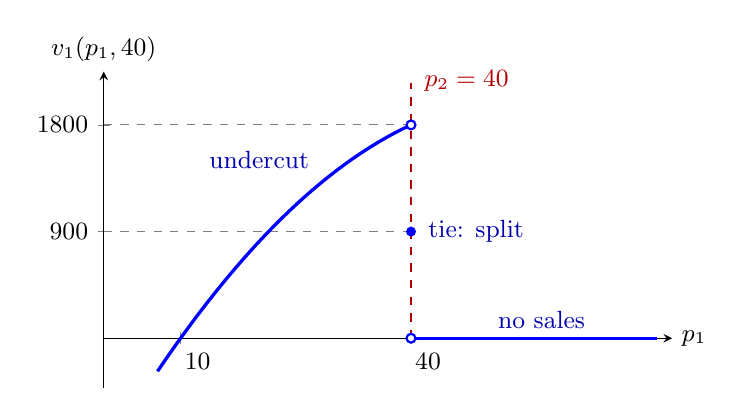
\begin{tikzpicture}[font=\small, >={Latex[length=2mm]}]
  \begin{axis}[
    axis lines=middle,
    xmin=0, xmax=74, ymin=-420, ymax=2250,
    xtick={10,40}, ytick={900,1800},
    xlabel={$p_1$}, ylabel={$v_1(p_1,40)$},
    xlabel style={anchor=west}, ylabel style={anchor=south},
    tick label style={font=\small},
    yticklabel style={/pgf/number format/1000 sep={}},
    xticklabel style={anchor=north west, xshift=-2pt},
    clip=false,
    width=8.8cm, height=5.6cm]
    % rival price
    \draw[red!70!black, dashed, thick] (axis cs:40,0) -- (axis cs:40,2150);
    \node[red!70!black, anchor=south west] at (axis cs:40.5,2000) {$p_2=40$};
    \draw[gray, thin, dashed] (axis cs:0,1800) -- (axis cs:40,1800);
    \draw[gray, thin, dashed] (axis cs:0,900) -- (axis cs:40,900);
    % firm 1's profit
    \addplot[blue, very thick, domain=7:40, samples=60] {(x-10)*(100-x)};
    \addplot[blue, very thick, domain=40:72, samples=2] {0};
    \draw[blue, thick, fill=white] (axis cs:40,1800) circle (1.6pt);
    \draw[blue, thick, fill=white] (axis cs:40,0) circle (1.6pt);
    \fill[blue] (axis cs:40,900) circle (1.8pt);
    \node[blue!70!black, anchor=west] at (axis cs:41,900) {tie: split};
    \node[blue!70!black, anchor=south east] at (axis cs:28,1350) {undercut};
    \node[blue!70!black, anchor=south] at (axis cs:57,0) {no sales};
  \end{axis}
\end{tikzpicture}
\end{document}
